\documentclass[lmodern, utf8, diplomski, numeric]{fer}
\usepackage{booktabs}

\begin{document}

\thesisnumber{1115}

\title{DUBOKE KONVOLUCIJSKE NEURONSKE MREŽE ZA RASPOZNAVANJE ZNAKOVA}

\author{Matija Ilijaš}

\maketitle

% Ispis stranice s napomenom o umetanju izvornika rada. Uklonite naredbu \izvornik ako želite izbaciti tu stranicu.
\izvornik

% Dodavanje zahvale ili prazne stranice. Ako ne želite dodati zahvalu, naredbu ostavite radi prazne stranice.
\zahvala{}

\tableofcontents

\chapter{Uvod}

Optičko prepoznavanje znakova  (eng. Optical Character Recognition – OCR) područje je istraživanja u računalnom vidu koje se bavi segmentacijom i klasifikacijom znakova sa slike. Prepoznavanje teksta sa slike ima vrlo široku primjenu u mnogim područjima ljudske djelatnosti. Jedna od trenutno najvećih primjena je arhiviranje i pretvorba dokumenata iz papirnatog oblika u digitalni oblik kako bi se mogli jednostavnije i brže pohranjivati i pretraživati. Razvijanjem mobilne tehnologije i njene primjene u svakodnevnom životu pojavljuju se nove izazovnije primjene optičkog prepoznavanja znakova koje zahtijevaju prepoznavanje teksta u prirodnim scenama. Tako se danas OCR algoritmi koriste za prepoznavanje podataka sa osobnih dokumenata i računa, prepoznavanje teksta za simultano prevođenje teksta, rješavanje matematičkih jednadžbi i mnoge druge primjene.

U strojnom učenju se u zadnjih nekoliko godina pojavilo novo obečavajuće područje istraživanja pod nazivom duboko učenje. Koncept dubokog učenja zasniva se na učenju korisnih prezentacija podataka povezanih u obliku hijerarhije, te je djelomično inspiriran vizualnim korteksom mozga sisavca. Zbog velike kompleksnosti modela dubokog učenja, te velike količine podataka potrebnih za učenje, istraživanja su u ovom području postala tek nedavno moguća uvođenjem specijaliziranih alata za brzo učenje na grafičkim karticama. Algoritmi dubokog učenja pokazali su jako dobre rezultate na problemima raspoznavanja uzoraka, posebice u području računalnog vida. Za problem klasifikacije na temelju slika razvijene su duboke konvolucijske neuronske mreže, također inspirirane vizualnim korteksom, koje su ostvarile najbolje rezultate na gotovo svim javno dostupnim skupovima za testiranje. Dodatni dokaz da duboko učenje u nekoj mjeri oponaša vizualni korteks su i nedavna istraživanja gdje su se značajke slike naučene dubokim učenjem pokazale sličnim onima u korteksu.

U ovom radu provedeno je istraživanje primjene dubokih konvolucijskih neuronskih mreža na problemu raspoznavanja znakova. U tu svrhu razvijen je sustav za učenje i testiranje različitih arhitektura standarnih neuronskih mreža te dubokih konvolucijskih neuronskih mreža. Podsustav za učenje implementiran je pomoću razvojnog alata za paralelno računanje na grafičkoj kartici kako bi postupak bio što brži. Dio sustava za testiranje razvijen je s ciljem detaljne analize rada naučenih modela, te jednostavne i pregledne usporedbe više različitih modela. 

Istraživanje je ostvareno uz dodatnu podršku tvrtke MicroBlink specijalizirane za razvoj tehnologija računalnog vida za mobilne uređaje. Za učenje i testiranje modela koriste se od tvrtke interni skupovi podataka, a prilikom testiranja provodi se analiza i njihovog internog klasifikatora. 
Rezultati su prikazani i komentirani sa ciljem pronalaska optimalne arhitekture modela za primjenu na mobilnom uređaju. Pritom je osim točnosti naučenih klasifikatora uzeta u obzir i njihova kompleksnost te prosječno trajanje klasifikacije.





\chapter{Optičko prepoznavanje znakova}

Proces optičkog prepoznavanja znakova provodi se u dva glavna koraka, segmentacije znakova iz slike i njihovog klasificiranja. U ovom radu provodi se istraživanje metoda klasifikacije, te se koristi već segmentirani skup znakova za učenje i testiranje klasifikatora. Stoga je u nastavku ovog poglavlja opisan drugi korak optičkog prepoznavanja znakova, njihovo klasificiranje.

Kao i kod svakog problema raspoznavanje uzoraka u računalnom vidu, transformacije ulaznih slika znakova nastale promjenjivim uvjetima okoline znatno otežavaju klasifikaciju. Promjenjiva pozadina znakova, moguća oštećenja i okluzije, te različita osvijetljenja prilikom slikanja mogu znatno promjeniti ulaznu sliku. Geometrijske transformacije posljedica su i različitih parametara kamere s kojom se slika, kao i pozicije kamere u odnosu na sliku prilikom slikanja.  
Kako bi se smanjio utjecaj transformacija ulazne slike, standarni je postupak korištenje neke metode predprocesiranja prije slanja slike klasifikatoru.

\section{Predprocesiranje slike znaka}

Cilj predprocesiranja je proslijediti klasifikatoru sliku sa jasno definiranim područjem koje predstavlja znak. Često korišten postupak za dobivanje takve slike je metoda binarizacije, odnosno ograničavanje vrijednosti svih piksela slike na vrijednosti 0 ili 1. Tako dobivene binarne slike često imaju šum koji može otežati klasifikaciju, stoga se nakon binarizacije slika dodatno obrađuje morfološkim operacijama.

\subsection{Binariziranje slike}

Proces binarizacije uspoređuje svaku vrijednost piksela ulazne slike sa definiranim pragom, te ukoliko je vrijednost veća dodjeljuje pikselu novu vrijednost 1, a u suprotnom vrijednost 0. Postoji više metoda definiranja praga za pojedinačni piksel. Najjednostavnija metoda binarizacije koristi ručno određeni prag fiksne vrijednosti jednak za sve piksele. Ovako definiran prag je teško odrediti zbog promjenjivog intenziteta piksela pozadine i znaka, stoga naprednije metode računaju prag na temelju ulazne slike. 

Jednostavniji pristup računanja praga koristi se svim vrijednostima piksela slike, te provodi binarizaciju piksela sa istim globalnim pragom. Ovako određen prag daje bolje rezultate od ručno određenog praga zbog bolje prilagođenosti pojedinačnoj slici, no zbog svoje fiksne vrijednosti za sve piksele nije robustan na lokalne promjene u kontrastu slike. 

Kako bi binarizacija bila robusna na promjene u osvijetljenju potrebno je određivati prag pojedinačno za svaki piksel u slici. Takav prag se zove adaptivni, te se računa na temelju lokalnog susjedstva piksela. Sama operacija računanja praga može biti jednostavni prosjek vrijednosti svih piksela u susjedstvu ili težinski prosjek koristeći se Gaussovom jezgrom.


\subsection{Morfološke operacije}

Digitalnom morfologijom analiziraju se oblici digitalnih objekata. Slika se promatra u kontekstu teorije skupova te se predstavlja kao skup binarnih elemenata koji su grupirani u određene dvodimenzionalne strukture. Za obrađivanje binarnih slika tipično se koriste morfološke operacije dilatacije i erozije, te njihovih kombinacija, operacija zatvaranja i otvaranja. 

Dilatacija prolazi sa strukturnim elementom po slici i traži maksimalnu vrijednost piksela zahvaćenog dijela slike. Pronađenu maksimalnu vrijednost postavlja kao vrijednost svojeg središnjeg piksela, te na taj način proširuje svijetle regije piksela na slici. Erozija, s druge strane, traži minimalnu vrijednost piksela te vrši isti postupak i proširuje tamne regije piksela. Binarna slika sadrži izdvojen znak u crnoj boji na bijeloj podlozi, odnosno predstavljena je tamnom regijom piksela okruženom svijetlim pikselima. Izdvojeni znak u nekim slučajevima ima problem preširokih rubova, odnosno prevelik broj tamnih piksela koji čine njegovo područje. Primjenom dilatacije dolazi do širenja svijetlih regija piksela koje okružuju znak te sužuju njegove rubove

S obzirom da je u praksi teško znati kada je potrebna dilatacija a kada erozija, češće se koriste njihove kombinacije, otvaranje i zatvaranje.
Operacija otvaranja primjenjuje prvo eroziju pa dilataciju na slici, čime uklanja nepotrebni šum na slici. Zatvaranje provodi prvo dilataciju slike a zatim eroziju, te uklanja mala oštećenja na objektima. 


\section{Klasifikacija slike znaka}

Kako bi odredili ASCII vrijednost znaka, potrebno je sliku znaka provesti kroz postupak klasifikacije. 


\chapter{Umjetne neuronske mreže}

Umjetna neuronska mreža je algoritam strojnog učenja inspiriran strukturom i funkcionalnošću ljudskog mozga. Zasniva se na paralelnoj obradi podataka, te vrlo dobro rješava probleme kod kojih postoji složena nelinearna veza ulaza i izlaza. Radi s velikim brojem parametara i varijabli, te može raditi s nejasnim podacima što ju čini robusnom na pogreške. Jedna od najčešćih primjena neuronskih mreža je u području raspoznavanja uzoraka.

Mreža se sastoji od tri vrste sloja: ulaznog, izlaznog, te skrivenog koji povezuje prethodna dva. Čvorišta, tzv. neuroni, skrivenog sloja povezani su težinskim vezama s ulaznim i izlaznim neuronima. Dvije su faze rada umjetnih neuronskih mreža: učenje (treniranje) i obrada podataka (eksploatacija). Učenje je iterativan postupak predočavanja ulaznih primjera i očekivanog izlaza pri čemu dolazi do postupnog prilagođavanja težina veza neurona. Nakon što se težine skrivenog sloja prilagode postupkom treniranja, eksploatacijom neuronske mreže može se za do tad neviđeni ulazni primjer dobiti pripadajući izlaz.

\section{Umjetni neuron}
\section{Učenje neuronskih mreža}


\chapter{Duboko učenje}

Duboko učenje se u zadnjih nekoliko godina pojavilo kao novo obečavajuće područje statističkog strojnog učenja. Iako je sama ideja prezentirana u radovima Yanna Lecuna i Georgea Hintona prije gotovo 30 godina, duboko učenje je postalo predmetom istraživanja relativno nedavno. Razlog tome su bila tada nedovoljno snažna računala za učenje velikih modela karakterističnih za taj pristup. Koncept dubokog učenja zasniva se na učenju korisnih prezentacija podataka povezanih u obliku hijerarhije. Ideja je djelomično inspirirana vizualnim korteksom mozga sisavaca koji se sastoji od niza procesirajućih elemenata koji obrađuju vizualni podražaj. Dokaz da duboko učenje u nekoj mjeri oponaša vizualni korteks su i nedavna istraživanja gdje su se naučene značajke pokazale slične onima u korteksu. Glavna karakteristika algoritama dubokog učenja je velik broj slojeva kroz koje ulazni podatak mora proći do izlaza, gdje se prvi dio prolaza može zamisliti kao formiranje hijerarhijskog prikaza podatka, a drugi kao proces klasifikacije. Time jedan algoritam dubokog učenja ustvari preuzima zadatak izvlačenja korisnih značajki iz podataka uz sami zadatak klasifikacije. Kod učenja takvog algoritma cijeli se postupak uči na temelju podataka, te se time gubi potreba za ručnim definiranjem značajki podataka. 

\section{Hijerarhijski prikaz podataka}

Slika se može klasifikatoru prikazati na mnogo načina, od kojih je najjednostavniji vektor vrijednosti intenziteta piksela. Apstraktniji prikaz bio bi recimo skup rubova na slici, a još apstraktniji skup različitih oblika. Neki prikazi olakšavaju klasifikatoru proces učenja, a različiti problemi klasifikacije zahtijevaju razvijanje različitih prikaza odnosno značajki ulaznih podataka. Stoga  se tradicionalno razvijanje rješenja problema klasifikacije sastoji od dva dijela, razvijanja kvalitetnih značajki koje olakšavaju učenje te razvijanja klasifikatora. 

Proces razvoja kvalitetnih značajki podrazumijeva promatranje svojstva ulaznih podataka te naglašavanje onih koja su maksimalno diskriminantna. Napredak u točnosti klasifikacije većim dijelom se ostvarivao razvijanjem boljih značajki, tako je na primjer značajni napredak u prepoznavanju čovjeka ostvaren razvijanjem HoG značajki koje su dobro opisivale lokalne oblike te u isto vrijeme bile invarijantne na  promjene osvijetljenja i geometrijske transformacije. No s obizrom da se takav postupak razvijanja značajki bazira na ljudskom promatranju podataka, dolazi do gubitka informacija koje čovjek nije u stanju vidjeti. 

Kako bi se koristile sve informacije iz podataka, potrebne su metode koje određuju diskriminantne značajke izravno iz skupa podataka. Među popularnijim metodama tog tipa su metoda linearne diskriminantne analize (LDA) te metoda glavnih komponenata (PCA). Linearna diskriminantna analiza pronalazi prikaz podataka koji maksimalno diskriminira podatke različitih klasa, dok metoda glavnih komponenata prikazuje podatke kao linearnu kombinaciju linearno nekoreliranih varijabli koje imaju najveću varijancu.

\begin{figure}[ht!]
\centering
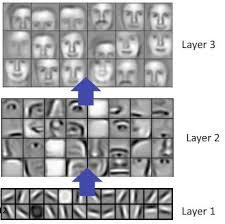
\includegraphics[height=9cm]{slike/feature_hierarchy2.jpeg}
\caption{}
\end{figure}

Istraživanja vizualnog korteksa mozga sisavaca pokazala su da vizualni podražaj prolazi kroz više procesirajućih slojeva koji tvore hijerarhiju gdje svaki dodatni sloj predstavlja dodatnu razinu apstrakcije.  Značajke dobivene prethodno navedenim metodama predstavljaju jednu razinu apstrakcije, te se mogu zamisliti kao imitacija najnižeg sloja vizualnog korteksa. Ideja dubokog učenja inspirirana je vizualnim korteksom te se zasniva na učenju cijele hijerarhije, odnosno više razina apstrakcije. Primjer jedne takve hijerarhije značajki ljudskog lica naučene dubokim učenjem prikazan je na Slici ???.


\section{Učenje dubokih mreža}

Kao što je ranije spomenuto ideja dubokog učenja je naučiti hijerarhiju značajki iz podataka. S obzirom da to zahtijeva nekoliko dodatnih slojeva mreže, kompleksnost dubokih modela značajno je veća od standarnih. Poznato je da količina potrebnih podataka za kvalitetno učenje modela raste proporcionalno sa brojem njegovih slobodnih parametara. Stoga je za učenje dubokih mreža potrebno za red veličine više podataka nego kod učenja standarnih klasifikatora. Nedovoljna količina podataka za učenje, te nedovoljno jaka računala za učenje tako velikih modela, razlog su zašto duboko učenje nije zaživjelo 1980-ih godina kada je prvi put predstavljeno kao ideja. Dolazak specijaliziranih razvojnih alata za brzo učenje mreža na grafičkim karticama, kao i sve veća količina dostupnih podataka za učenje, omogućili su da duboko učenje u zadnjih nekoliko godina pokaže svoj potencijal na raznim problemima strojnog učenja.

Jedna od velikih prednosti dubokog učenja je što uz metode nadziranog učenja ima razvijene i metode nenadziranog učenja. U ovom radu koristi se isključivo nadzirano učenje zbog dostupnosti velike količine označenih podataka. U nastavku ovog poglavlja opisana je metoda nenadziranog učenja, a metoda nadziranog učenja opisana je u idućem poglavlju kao uvod u duboke konvolucijske mreže.

Sve veća količina podataka postaje dostupna za učenje, no velikim dijelom radi se o neoznačenim podatcima. Kako bi se i ti podatci iskoristili potrebne su metode nenadziranog učenja. Kao što je ranije spomenuto, duboki modeli predstavljaju hijerarhiju značajki podataka, a jednu razinu apstrakcije moguće je postići metodom glavnih komponenata (PCA). Stoga se u teoriji postavlja pitanje da li uzastopnim primjenjivanjem metode glavnih komponenata možemo dobiti traženu hijerarhiju. Odgovor na to pitanje je da ne možemo, a razlog tome je linearnost te metode. Uzastopnom linearnom transformacijom konačno se uvijek dobiva linearna transformacija, što onemogućuje stvaranje željene hijerarhije. Iz tog razloga razvijene su dvije nove metode sa dodanom nelinearnošću, autoenkoderi i ograničeni Boltzmann strojevi. U sklopu ovog rada opisati će se autoenkoderi, jednostavnija i intuitivnija metoda od dvije navedene.

Autoenkoder je jednostavna troslojna neuronska mreža kod koje su izlazni neuroni izravno povezani sa ulaznim neuronima. 

\begin{figure}[ht!]
\centering
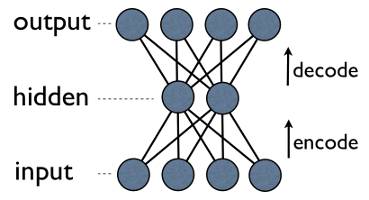
\includegraphics[width=9cm]{slike/autoenkoder.png}
\caption{}
\end{figure}

Broj neurona u srednjem sloju manji je od onog u ulaznom i izlaznom sloju. Kao posljedica toga prolaskom podataka kroz mrežu događaju se dvije radnje, enkodiranje i dekodiranje. Zato što je broj neurona srednjeg sloja manji od broja elemenata ulaznog sloja, ulazni vektor se kompresira, odnosno podatak se u srednjem sloju prikazuje pomoću apstraktnijih značajki. Nakon toga vrši se dekompresija, odnosno dekodiranje, kako bi se na temelju značajki iz srednjeg sloja rekonstruirao ulazni vektor.
Vrijednosti izlaznog vektora zatim se uspoređuju sa onima ulaznog vektora kako bi se dobila informacija o kvaliteti rekonstrukcije, odnosno koliko dobro značajke iz srednjeg sloja predstavljaju ulazni podatak.

Proces učenja autoenkodera sastoji se od iterativnog enkodiranja i dekodiranja ulaznih podataka za učenje te korigiranja njegovih težina na temelju greške u rekonstrukciji. Rezultat učenja je autoenkoder sa težinama koje čine elemente njegovog srednjeg sloja apstraktnim značajkama koje dobro opisuju prezentirane podatke. 

S obzirom da autoenkoder radi nelinearnu transformaciju nad ulaznim podatcima, možemo ostvariti hijerarhiju apstraktnih značajki slijednim povezivanjem više autoenkodera. Učenje se provodi iterativno, odnosno prvi autoenkoder uči se na temelju ulaznih podataka, a svaki idući na temelju naučenih značajki svojeg prethodnika. 

\begin{figure}[ht!]	
\centering
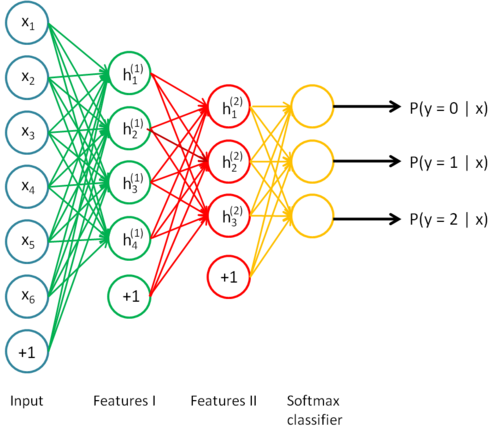
\includegraphics[width=9cm]{slike/stacked_autoencoders.png}
\caption{}
\end{figure}

Ovako dobivena mreža naučena je isključivo na neoznačenim podatcima te predstavlja hijerarhiju značajki podataka bez mogućnosti klasifikacije. Konačni klasifikator dobiva se dodavanjem jedne manje mreže koja na ulaz prima značajke zadnjeg autoenkodera a na izlaz vraća klase zadanog problema. Tako povezana mreža autoenkodera i mreža za klasifikaciju zatim se uče na označenim podatcima kao jedna velika mreža.


\chapter{Duboke konvolucijske neuronske mreže}

U prethodnom poglavlju opisana je metoda nenadziranog učenja koja može naučiti hijerarhiju značajki koristeći se neoznačenim podatcima, a zatim naučiti klasificirati pomoću manjeg skupa označenih podataka. Ovaj pristup je praktičan u većini problemskih domena zbog male količine dostupnih označenih podataka za učenje. No u praksi se pokazalo da za određene probleme, gdje ima dovoljno označenih podataka, najbolje rezultate daju metode nadziranog učenja. Problemska domena ovog rada ima dostupnu veliku količinu označenih podataka, te su svi modeli učeni metodama nadziranog učenja.

Kao i kod nenadziranog učenja, konačni model koji se uči sastoji se od dijela za formiranje hijerarhije značajki i dijela za klasifikaciju, no nadzirano učenje je proces koji se provodi u jednom koraku i na jednom skupu podataka. Sam postupak učenja ne razlikuje se od standarnog učenja neuronske mreže metodom gradijentnog spusta.

Istraživanja vizualnog korteksa pokazala su da njegovi procesirajući elementi reagiraju na male lokalne podražaje unutar vizualnog polja, funkcionirajući kao lokalni receptori. Glavna karakteristika prirodnih slika je njihova lokalna prostorna korelacija, pa je logično da se vizualni korteks prilagodio traženju lokalnih značajki.
Klasične neuronske mreže sa potpuno povezanim slojevima ne iskorištavaju ovo korisno svojstvo, stoga je razvijena konvolucijska neuronska mreža koja sa svojim lokalnim prostornim filterima oponaša lokalne receptore vizualnog korteksa.

\section{Lokalni prostorni filteri}

Konvolucijom ostvareni filteri omogućuju provođenje kompleksnih operacija jednostavnom promjenom konvolucijske jezgre. Tako bi na primjer upotrebom Gaussian jezgre dobili za rezultat zamućenje slike, a upotrebom Sobel jezgre naglašene rubove na slici. Ručno definiranje konvolucijskih jezgri upravo odgovara ranije spomenutom ručnom određivanju značajki u standarnom postupku razvijanja klasifikatora. Cilj konvolucijske neuronske mreže je naučiti konvolucijske jezgre specifične za dane podatke, što odgovara ranije spomenutom učenju značajki iz podataka.

U dubokoj konvolucijskoj mreži prvih nekoliko slojeva zaduženih za izgradnju hijerarhije značajki je konvolucijsko. Uloga prvog sloja konvolucije je jasna s obzirom da odgovara standarnom filtriranju slike sa nekom konvolucijskom jezgrom. Viši slojevi konvolucije nemaju doticaja sa ulaznom slikom, već formiraju apstraktnije lokalne značajke od značajki prethodnog sloja. Na primjer u problemu detekcije čovjeka prvi sloj konvolucije razvio bi lokalne detektore rubova na slici, sloj iznad njega formirao bi lokalne oblike koristeći se sa rubovima iz prvog sloja, a sloj za razinu više bi koristio lokalne oblike za formiranje detektora dijelova tijela čovjeka. Jednom kada mreža ima detektore značajki koje opisuju prisutnost glavnih dijelova objekta, u ovom slučaju čovjeka, klasifikacija postaje jednostavna.

\begin{figure}[ht!]
\centering
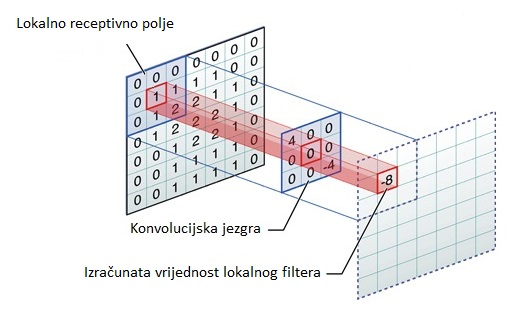
\includegraphics[width=14cm]{slike/kernel_convolution.jpg}
\caption{}
\end{figure}

\section{Dijeljenje težina}

Jednom naučeni lokalni filteri mogu prepoznati neku značajku podataka, no nepoznato je gdje se ta značajka nalazi u prostoru. Kako bi razvili lokalne filtere invarijantne na poziciju u prostoru, potrebno je za svaki filter imati skup njegovih inačica koje pokrivaju sve moguće podprostore. Takav skup zovemo mapa značajki, a glavna karakteristika takve mape je dijeljenje težina između svih elemenata skupa. Svaki element konvolucijskog sloja prikazuje se tada kao matrica koja sadrži vrijednosti odziva  pripadajućeg filtera za svaku poziciju u prostoru. Primjer jedne takve mape značajki na višoj razini apstrakciji prikazan je na Slici ???, gdje je važno primjetiti da konvolucija nakon prvog sloja postaje trodimenzionalna zbog uvođenja mape značajki koja je dvodimenzionalni prikaz elementa konvolucijskog sloja.

\begin{figure}[ht!]
\centering
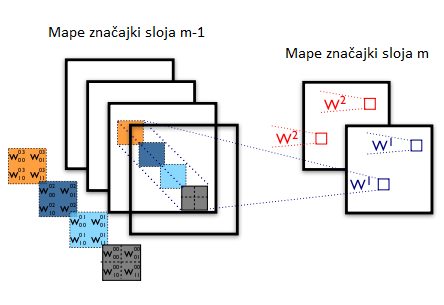
\includegraphics[width=12cm]{slike/shared_weights.png}
\caption{}
\end{figure}

Za učenje mreža sa dijeljenim težinama još uvijek se može koristiti metoda gradijentnog spusta, ali uz malu preinaku. Gradijent dijeljene težine računa se kao suma gradijenata svih parametara koji se dijele. 
Osim što ostvaruje prostornu invarijantnost lokalnih filtera, dijeljenje težina znatno doprinosi i procesu učenja konvolucijske mreže. Dijeljenjem težina između parametara  mreže smanjujemo ukupan broj slobodnih parametara koje je potrebno naučiti, što smanjuje trajanje učenja. No ono što je još važnije, smanjenjem slobodnih parametara poboljšava se sposobnost generalizacije mreže stavljanjem dodatnog ograničenja na njenu kompleksnost.  

\section{Lokalno udruživanje}

Još jedan važan koncept dubokih konvolucijskih mreža je lokalno udruživanje, koje se može definirati kao oblik nelinearnog poduzorkovanja. U praksi se najviše koristi inačica maksimalnog lokalnog udruživanja (eng. max pooling) koja za poduzorkovanje koristi operaciju traženja maksimuma. 
Postupak maksimalnog lokalnog udruživanja na slici sastoji se od dijeljenja slike na nepreklapajuće podprozore fiksne veličine, te uzimanja maksimalne vrijednosti svakog podprozora za rezultat. Dobivena slika za podprozore veličine 2x2 bila bi u tom slučaju dvostruko manja od originalne slike, sa vrijednostima svih maksimalnih elemenata podprozora. 
Maksimalno lokalno udruživanje se u dubokim konvolucijskim mrežama ne primjenjuje na ulaznoj slici, već kao dodatni sloj nakon svakog sloja konvolucije. Time ova metoda postaje korisna na dva načina: eliminira vrijednosti koje nisu maksimalne što smanjuje količinu računanja u višim slojevima, te ostvaruje jedan oblik invarijantnosti na translaciju. Invarijantnost proizlazi iz činjenice da se uzimanjem maksimalne vrijednosti nekog podprozora prepoznaje odziv lokalnog filtera na bilo kojoj lokaciji unutar podprozora, odnosno dopušta se mali pomak naučenih značajki u prostoru.


\begin{figure}[ht!]
\centering
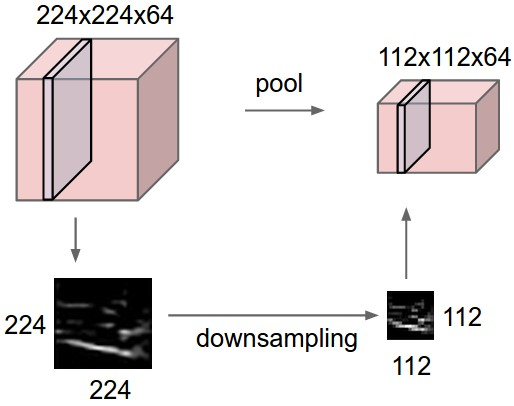
\includegraphics[width=10cm]{slike/max_pooling.jpeg}
\caption{}
\end{figure}


\section{Ispravljena linearna jedinica}

Ono što razlikuje neuronske mreže od linearnih klasifikatora su dodane prijenosne funkcije za postizanje nelinearnosti. U standarnoj potpuno povezanoj neuronskoj mreži svaki element sadrži prijenosnu funkciju, najčešće sigmoidalnog tipa. Dodavanje nelinearnosti u dubokoj konvolucijskoj mreži postiže se dodavanjem sloja koji na svaku vrijednost prijašnjeg sloja primjenjuje prijenosnu funkciju. 

Primjenom sigmoidalne prijenosne funkcije kod učenja duboke arhitekture pojavljuje se problem nestajućeg gradijenta. Zbog svojstva sigmoidalne funkcije da ograničava vrijednosti na mali izlazni interval, vrijednosti gradijenata postaju izrazito male ukoliko se prosljeđuju kroz veliki broj slojeva, što onemogućuje kvalitetno učenje.
Rješenje ovog problema je osmišljeno primjenom ispravljene linearne jedinice kao prijenosne funkcije. Ispravljena prijenosna funkcija definirana je operacijom maksimuma od ulazne vrijednosti i nule, što ju čini izrazito jednostavnom za računanje. Osim što se rješava problem nestajućeg gradijenta, postiže se i efekt raspršene aktivacije, odnosno u prosjeku se samo pola elemenata aktivira svakim prolazom kroz mrežu što pospješuje sposobnost generalizacije.  

\begin{figure}[ht!]
\centering
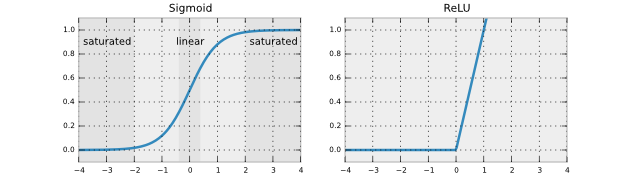
\includegraphics[width=15cm]{slike/sigmoid_relu.png}
\caption{}
\end{figure}


\section{Konačni model}

Kao što je ranije spomenuto, konačni model duboke konvolucijske mreže sastoji se od dijela za formiranje hijerarhije značajki i dijela za klasifikaciju. Prvi dio modela ostvaren je slojevima koji implementiraju ranije spomenute koncepte dubokih konvolucijskih mreža, a drugi standardnim potpuno povezanima slojevima. 

Nakon svakog sloja konvolucije dodaje se sloj maksimalnog lokalnog udruživanja, a zatim sloj ispravljenih linearnih jedinica za postizanje nelinarnosti. Primjer jednog takvog konačnog modela prikazan je na Slici ???.

\begin{figure}[ht!]
\centering
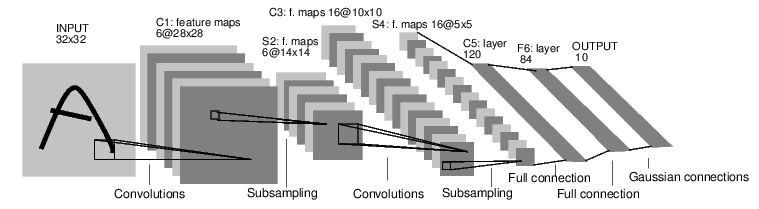
\includegraphics[width=15cm]{slike/convnet2.png}
\caption{}
\end{figure}

Odabir arhitekture dubokih konvolucijskih mreža dodatno je otežan u odnosu na standarne neuronske mreže. Osim standarnih hiperparametara koji određuju broj slojeva i broj elemenata po sloju mreže, za duboku konvolucijsku arhitekturu potrebno je odrediti veličine lokalnih prostornih filtera i filtera maksimalnog lokalnog udruživanja. Veličine lokalnih filtera ponajprije ovise o veličine ulazne slike, te je cilj odrediti veličinu kojom će se kvalitetno formirati apstrakcije po slojevima. Veličine filtera maksimalnog lokalnog udruživanja uobičajeno su male zbog gubljenja velike količine podataka kod većih filtera. Također je važno uzeti u obzir da se veličine mapa značajki smanjuju nakon svakog sloja konvolucije i lokalnog udruživanja, što se u praksi kompenzira dodavanjem većeg broj mapa u višim slojevima.



\chapter{Implementacija}

U sklopu ovog rada razvijen je sustav za učenje i testiranje različitih arhitektura neuronskih mreža. Prilikom razvijanja takvog sustava bilo je važno zadovoljiti dva glavna uvjeta: brzo učenje novih arhitektura na velikoj količini podataka te detaljna analiza rada naučenih mreža. Iz tog razloga sustav je podijeljen na dva podsustava razvijena sa zasebnim alatima. Podsustav zadužen za učenje implementiran je u razvojnom alatu Torch koji omogućuje paralelno izvođenje procesa učenja na grafičkoj kartici. Podsustav koji provodi analizu rada naučenih mreža implementiran je u jeziku C++ korištenjem OpenCV biblioteke.

\section{Sustav za učenje}

Kako bi cijeli proces istraživanja različitih arhitektura mreža i podataka bio što efikasniji, potrebno je prije svega imati brz sustav za učenje. Učenje velikih arhitektura na velikoj količini podataka može trajati tjednima, pa i mjesecima, sekvencijalnim računanjem na standarnom procesoru računala. Stoga je tek pojavom specijaliziranih biblioteka koje omogućuju optimizirano paralelno računanje na grafičkoj kartici postalo moguće provoditi istraživanje u području dubokog učenja. 
Osim brzine učenja, važna je i jednostavnost definiranja parametara mreže koja se uči, kao i parametara samog procesa učenja. Kod implementacije ovog rada odabran je razvojni alat Torch zbog svoje jednostavnosti i brzine, ali i podrške velikih kompanija kao što su Facebook i Google, koje nerijetko dijele korisne implementacije sa zajednicom. 

\subsection{Torch razvojni alat}

Prilikom odabira razvojnog alata uzeti su u obzir i alati Caffe i Theano. Možda najpopularniji alat za duboko učenje Caffe ima izrazito jednostavno sučelje za odabir parametara mreže i procesa učenja, no kao posljedica toga teško je raditi promjene u postojećoj implementaciji u svrhu istraživanja ili razvoja. Theano s druge strane pruža puno manju razinu apstrakcije te ostavlja mogućnost lake izmjene većine implementacije, no postaje nepraktičan kod česte upotrebe standarnih algoritama.
Torch je po razini apstrakcije negdje između prethodno navedenih alata, dovoljno je niske apstrakcije za laku izmjenu implementacije kod razvoja i istraživanja, ali ima i sučelje za standarne algoritme koje ga čini praktičnim. 

Brzina samog izvođenja procesa učenja na grafičkim karticama velikim dijelom ovisi o pozadinskoj implementaciji paralelnog računanja koja je za sve navedene alate otprilike podjednako brza, te se toliko često mijenja da nema smisla uspoređivati njihove brzine. S druge strane, važan faktor kod odabira alata je podrška akademske zajednice i industrije s obzirom da o tome ovisi koliko brzo se razvijaju implementacije novih koncepata. Torch ima implementaciju za većinu novih koncepata u dubokom učenju zbog podrške kompanija kao što su Google, Facebook i Twitter.  Tako je primjerice implementirana relativno nova metoda Dropout za regularizaciju prilikom učenja mreže te ReLU funkcija prijelaza koja je pokazale bolje rezultate od standardne sigmoidalne funkcije u nedavnim istraživanjima.

Sama implementacija Torcha podijeljena je na dva dijela. Sve računske operacije na grafičkoj kartici napisane su kao C/CUDA implementacija za maksimalnu brzinu, dok je ostatak funkcionalnosti implementiran u skriptnom jeziku LuaJIT za lakše korištenje alata.  

\subsection{Definiranje arhitekture}
	
Neuronska mreža je u Torch alatu definirana kao model koji se sastoji od sekvencijalno povezanih slojeva koji vrše različite računske operacije.
Tako bi na primjer standarna neuronska mreža s jednim skrivenim slojem bila definirana kao sekvencijalni niz prikazan na Slici ???. 

\begin{figure}[ht!]
\centering
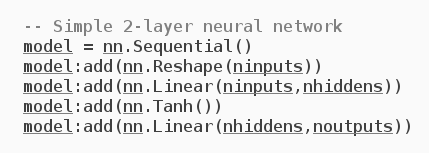
\includegraphics[width=9cm]{slike/nn_model.png}
\caption{}
\end{figure}

Primjer duboke konvolucijske mreže definirane kao Torch model prikazan je na Slici ???.

\begin{figure}[ht!]
\centering
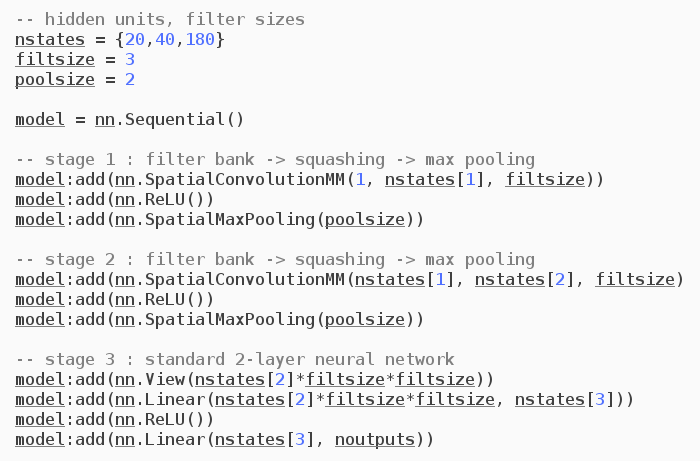
\includegraphics[width=16cm]{slike/cnn_model.png}
\caption{}
\end{figure}

\subsection{Definiranje parametara učenja}




\section{Sustav za testiranje}

Detaljna analiza rada naučenih mreža ključna je za pronalaženje optimalne arhitekture. Mjera optimalnosti nekog modela općenito se može definirati kao omjer njegove točnosti klasifikacije i njegove kompleksnosti. Ovisno o području primjene postoje određena ograničenja i prioriteti za različite karakteristike modela. U ovom radu razvijen je sustav koji analizira naučene mreže u dovoljno detalja da bi se donosili kvalitetni zaključci o njihovoj primjenjivosti. Osim analize pojedinih modela omogućeno je i simultano analiziranje više modela za što lakšu usporedbu njihovih pojedinih karakteristika.  

\subsection{Matrica greške klasifikacije}

Testiranjem klasifikatora na skupu podataka u konačnici se dobivaju dvije oznake klasa za svaki podatak. Jedna oznaka je ručno određena te uvijek predstavlja točnu klasu podatka, dok drugu dobivamo kao rezultat klasifikatora koji se testira. Standarna mjera točnosti klasifikatora koristi se dobivenim oznakama samo za informaciju o tome da li oznaka klasifikatora odgovara označenoj oznaci, te vraća kao informaciju ukupni postotak točno klasificiranih podataka. Promatranjem klasa oznaka koje klasifikator vraća u slučaju krive klasifikacije može se dobiti bolji uvid u rad analiziranog modela. 
Matrica greške klasifikacije definirana je redovima koji predstavljaju ručne oznake klasa, te stupcima koji predstavljaju oznake dobivene klasifikatorom. Matrica se generira brojanjem uređenih parova ručne oznake i oznake klasifikatora, odnosno tražene i dobivene oznake. Tako bi na primjer potpuno točan klasifikator generirao matricu sa vrijednostima nula na svim mjestima osim na glavnoj dijagonali matrice gdje su tražene i dobivene oznake jednake.
Ovakav prikaz greške klasifikacije omogućuje uvid u točnost klasifikatora za pojedine klase, kao i informaciju o klasama koje se često međusobno zamjenjuju.

\begin{figure}[ht!]
\centering
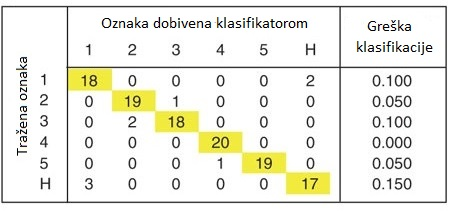
\includegraphics[width=13cm]{slike/confusion_matrix.jpg}
\caption{}
\end{figure}

\subsection{Prosječno trajanje klasifikacije}

Kako bi se donio zaključak o primjenjivosti nekog modela potrebno je poznavati i mjeru njegove kompleksnosti. Sustav za testiranje računa za svaku arhitekturu ukupan broj računskih operacija potrebnih za klasifikaciju jednog podatka. Kod standarnih potpuno povezanih mreža taj broj odgovara ukupnom broju veza između neurona, dok se kod kovolucijskih arhitektura uzimaju u obzir veličine filtera i mjere njihovog preklapanja. 

Kompleksnost modela se može definirati i brojem slobodnih parametara, koji je kod potpuno povezanih mreža jednak broju računskih operacija. Kod dubokih konvolucijskih arhitektura taj je broj manji od broja računskih operacija zbog ranije opisane metode dijeljenja težina lokalnih filtera, te se koristi za procjenu sposobnosti generalizacije klasifikatora.

Iako se pomoću broja računskih operacija može aproksimirati prosječno trajanje klasifikacije, sustav za testiranje provodi i empirijsko mjerenje. Testiranjem klasifikatora na skupu podataka bilježi se trajanje svake klasifikacije, što nam između ostalog omogućuje i računanje prosječnog trajanja klasifikacije.

\subsection{Simultano analiziranje više modela}

Osim analize pojedinih modela, sustav za testiranje omogućuje i simultano analiziranje više modela s ciljem njihove lakše usporedbe. Kod simultanog analiziranja prikazuju se sve ranije navedene informacije za svaki pojedini model, uz dodatak tabličnih prikaza pojedinih karakteristika svih modela. 

Kako bi rezultati bili što pregledniji, nakon analize svih modela generiraju se dva tablična prikaza. Prva tablica omogućuje lako uspoređivanje točnosti klasifikatora po pojedinim klasama i njihove ukupne točnosti. Druga tablica prikazuje prosječno trajanje klasifikacije za svaki analizirani model. 

Kod problema klasifikacije slika analizu znatno olakšava mogućnost vizualne provjere podataka. Vrlo često se može donijeti neki zaključak o slabostima klasifikatora promatranjem slika krivo klasificiranih primjera. Sustav za testiranje sprema za svaki analizirani model krivo klasificirane slike u zasebne datoteke ovisno o krivo određenoj klasi.






\chapter{Rezultati}

\chapter{Zaključak}
Zaključak.

\bibliography{literatura}
\bibliographystyle{fer}

\begin{sazetak}


\kljucnerijeci{Ključne riječi, odvojene zarezima.}
\end{sazetak}

\engtitle{Deep convolutional neural networks for character recognition}
\begin{abstract}
Abstract.

\keywords{Keywords.}
\end{abstract}

\end{document}
